%% This file was auto-generated by IPython.
%% Conversion from the original notebook file:
%%
\documentclass[11pt,english]{article}

%% This is the automatic preamble used by IPython.  Note that it does *not*
%% include a documentclass declaration, that is added at runtime to the overall
%% document.

\usepackage{amsmath}
\usepackage{amssymb}
\usepackage{graphicx}
\usepackage{grffile}
\usepackage{ucs}
\usepackage[utf8x]{inputenc}
\usepackage{float}

% Scale down larger images
\usepackage[export]{adjustbox}

%fancy verbatim
\usepackage{fancyvrb}
% needed for markdown enumerations to work
\usepackage{enumerate}

% Slightly bigger margins than the latex defaults
\usepackage{geometry}
\geometry{verbose,tmargin=3cm,bmargin=3cm,lmargin=2.5cm,rmargin=2.5cm}

% Define a few colors for use in code, links and cell shading
\usepackage{color}
\definecolor{orange}{cmyk}{0,0.4,0.8,0.2}
\definecolor{darkorange}{rgb}{.71,0.21,0.01}
\definecolor{darkgreen}{rgb}{.12,.54,.11}
\definecolor{myteal}{rgb}{.26, .44, .56}
\definecolor{gray}{gray}{0.45}
\definecolor{lightgray}{gray}{.95}
\definecolor{mediumgray}{gray}{.8}
\definecolor{inputbackground}{rgb}{.95, .95, .85}
\definecolor{outputbackground}{rgb}{.95, .95, .95}
\definecolor{traceback}{rgb}{1, .95, .95}

% new ansi colors
\definecolor{brown}{rgb}{0.54,0.27,0.07}
\definecolor{purple}{rgb}{0.5,0.0,0.5}
\definecolor{darkgray}{gray}{0.25}
\definecolor{lightred}{rgb}{1.0,0.39,0.28}
\definecolor{lightgreen}{rgb}{0.48,0.99,0.0}
\definecolor{lightblue}{rgb}{0.53,0.81,0.92}
\definecolor{lightpurple}{rgb}{0.87,0.63,0.87}
\definecolor{lightcyan}{rgb}{0.5,1.0,0.83}

% Framed environments for code cells (inputs, outputs, errors, ...).  The
% various uses of \unskip (or not) at the end were fine-tuned by hand, so don't
% randomly change them unless you're sure of the effect it will have.
\usepackage{framed}

% remove extraneous vertical space in boxes
\setlength\fboxsep{0pt}

% codecell is the whole input+output set of blocks that a Code cell can
% generate.

% TODO: unfortunately, it seems that using a framed codecell environment breaks
% the ability of the frames inside of it to be broken across pages.  This
% causes at least the problem of having lots of empty space at the bottom of
% pages as new frames are moved to the next page, and if a single frame is too
% long to fit on a page, will completely stop latex from compiling the
% document.  So unless we figure out a solution to this, we'll have to instead
% leave the codecell env. as empty.  I'm keeping the original codecell
% definition here (a thin vertical bar) for reference, in case we find a
% solution to the page break issue.

%% \newenvironment{codecell}{%
%%     \def\FrameCommand{\color{mediumgray} \vrule width 1pt \hspace{5pt}}%
%%    \MakeFramed{\vspace{-0.5em}}}
%%  {\unskip\endMakeFramed}

% For now, make this a no-op...
\newenvironment{codecell}{}

 \newenvironment{codeinput}{%
   \def\FrameCommand{\colorbox{inputbackground}}%
   \MakeFramed{\advance\hsize-\width \FrameRestore}}
 {\unskip\endMakeFramed}

\newenvironment{codeoutput}{%
   \def\FrameCommand{\colorbox{outputbackground}}%
   \vspace{-1.4em}
   \MakeFramed{\advance\hsize-\width \FrameRestore}}
 {\unskip\medskip\endMakeFramed}

\newenvironment{traceback}{%
   \def\FrameCommand{\colorbox{traceback}}%
   \MakeFramed{\advance\hsize-\width \FrameRestore}}
 {\endMakeFramed}

% Use and configure listings package for nicely formatted code
\usepackage{listingsutf8}
\lstset{
  language=python,
  inputencoding=utf8x,
  extendedchars=\true,
  aboveskip=\smallskipamount,
  belowskip=\smallskipamount,
  xleftmargin=2mm,
  breaklines=true,
  basicstyle=\small \ttfamily,
  showstringspaces=false,
  keywordstyle=\color{blue}\bfseries,
  commentstyle=\color{myteal},
  stringstyle=\color{darkgreen},
  identifierstyle=\color{darkorange},
  columns=fullflexible,  % tighter character kerning, like verb
}

% The hyperref package gives us a pdf with properly built
% internal navigation ('pdf bookmarks' for the table of contents,
% internal cross-reference links, web links for URLs, etc.)
\usepackage{hyperref}
\hypersetup{
  breaklinks=true,  % so long urls are correctly broken across lines
  colorlinks=true,
  urlcolor=blue,
  linkcolor=darkorange,
  citecolor=darkgreen,
  }

% hardcode size of all verbatim environments to be a bit smaller
\makeatletter 
\g@addto@macro\@verbatim\small\topsep=0.5em\partopsep=0pt
\makeatother 

% Prevent overflowing lines due to urls and other hard-to-break entities.
\sloppy

\linespread{2}


\title{A 1D Spherical $S_N$ Code with Diffusion Synthetic Acceleration}
\date{April 28, 2016}
\author{Pablo A. Vaquer\\ Texas A$\&$M University}

\begin{document}

\maketitle

\section{}

\subsection{}

The 1D spherical $S_N$ code was used to solve for the scalar flux using an isotropic incident flux. The solution is shown in Fig.(1).
\begin{figure}[!htb]
    \centering
    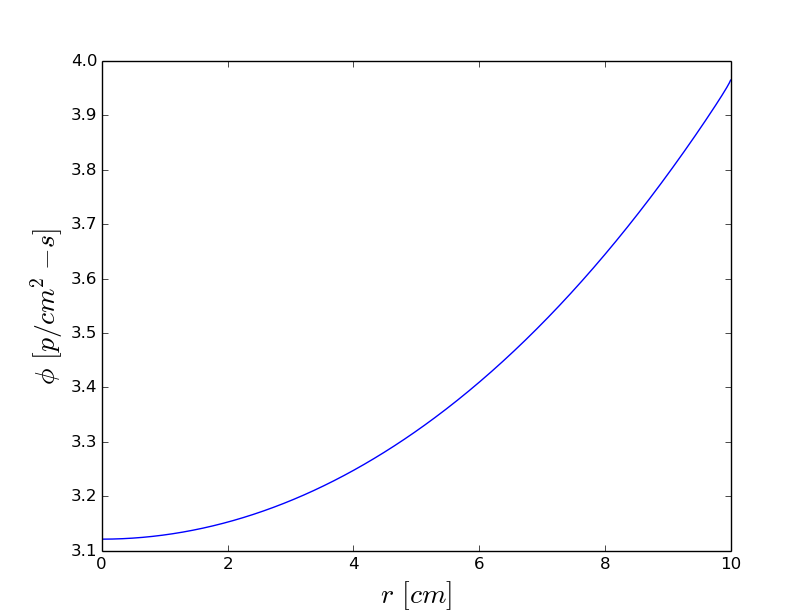
\includegraphics[width=0.6\textwidth]{final_1a.png}
    \caption{Scalar flux as a function of $r$ for part a}
    \label{fig:final_1a}
\end{figure}

\subsection{}

The 1D spherical $S_N$ code was used to solve for the scalar flux, using a delta-function distribution for the incident angular flux. The solution is shown in Fig.(2). The rapid variation in the solution near the boundary is called the ``boundary layer".
\begin{figure}[!htb]
    \centering
    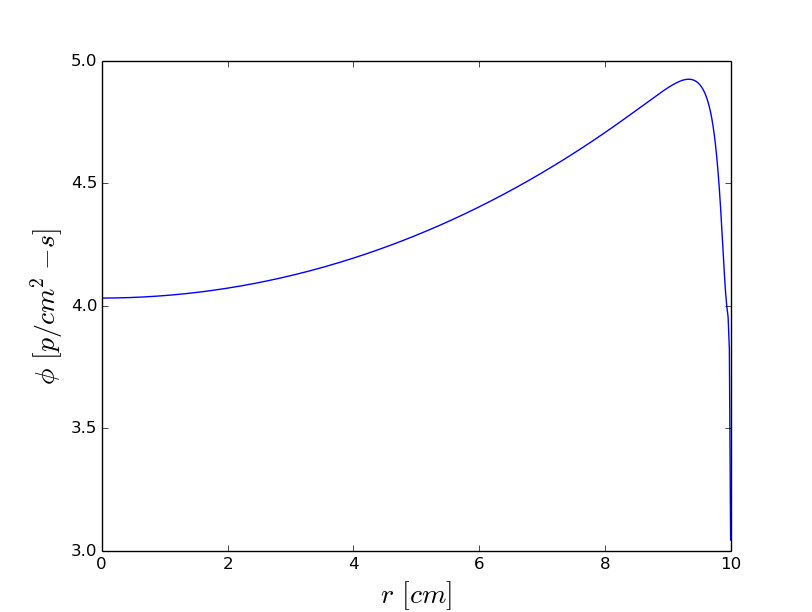
\includegraphics[width=0.6\textwidth]{final_1b.png}
    \caption{Scalar flux as a function of $r$ for part b}
    \label{fig:final_1b}
\end{figure}

\pagebreak

\subsection{}

For the boundary layer, the leading-order diffusion-limit solution is approximately
\begin{equation*}
\phi_B = \int_{-1}^0 d\mu \, (3\mu^2 + 2\mu) f(\mu) 
\end{equation*}
where 
\begin{equation*}
f(\mu) = C \, \delta(\mu - \mu_1) \: .
\end{equation*}
In addition, we know that the incident partial current on the right boundary is 1, thus we can solve for the constant $C$,
\begin{equation*}
J^- = 1 = \int_{-1}^0 d\mu \, \mu f(\mu) 
\end{equation*}
\begin{equation*}
1 = \int_{-1}^0 d\mu \, \mu C \delta(\mu - \mu_1) 
\end{equation*}
\begin{equation*}
C= \frac{1}{\mu_1}  \: .
\end{equation*}
Thus, 
\begin{equation*}
f(\mu) = \frac{\delta(\mu - \mu_1) }{\mu_1} \: . 
\end{equation*}
By plugging our updated $f(\mu)$ into our equation for $\phi_B$, we get
\begin{equation*}
\phi_B = \int_{-1}^0 d\mu \, (3\mu^2 + 2\mu) \frac{\delta(\mu - \mu_1) }{\mu_1} 
\end{equation*}
\begin{equation*}
\phi_B =  3 |\mu_1| + 2 
\end{equation*}
\begin{equation*}
\phi_B =  4.968
\end{equation*}
This is far from the value of $\phi_B = 2.839$ provided by the $S_N$ code. However, by doing a least-squares fit to the flux values between $0$ and $9$ cm we get the extrapolated value on the boundary would be $5.097$, this is within $2.5\%$ of the analytical value. The $S_N$ solution and the least-squares extrapolated solution are both shown in Fig.(3).

\begin{figure}[!htb]
    \centering
    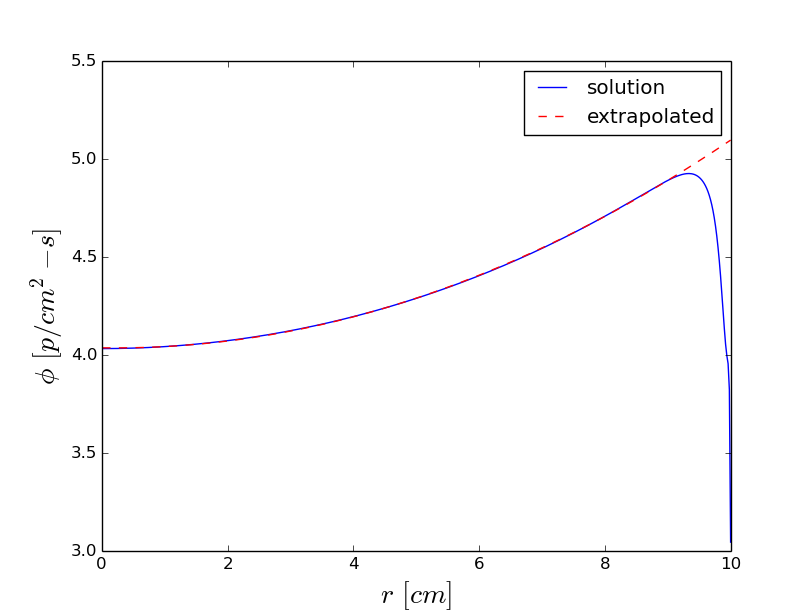
\includegraphics[width=0.6\textwidth]{final_1c.png}
    \caption{Scalar flux as a function of $r$ for part c}
    \label{fig:final_1c}
\end{figure}

\pagebreak 

\subsection{}

The $S_N$ code was used to solve for the scalar flux with only 10 cells, using an isotropic incident flux. This solution was compared to the solution for part a, shown in Fig.(4).
\begin{figure}[!htb]
    \centering
    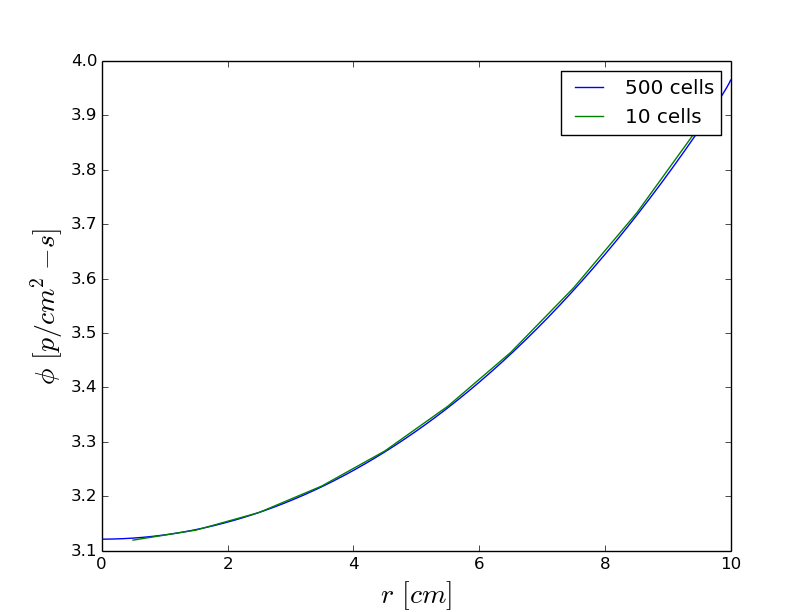
\includegraphics[width=0.6\textwidth]{final_1d.png}
    \caption{Scalar flux as a function of $r$ for part d}
    \label{fig:final_1d}
\end{figure}

\subsection{}

The $S_N$ code was used to solve for the scalar flux with only 10 cells, using a delta-function distribution for the incident angular flux. This solution was compared to the solution for part b, shown in Fig.(5).

\begin{figure}[!htb]
    \centering
    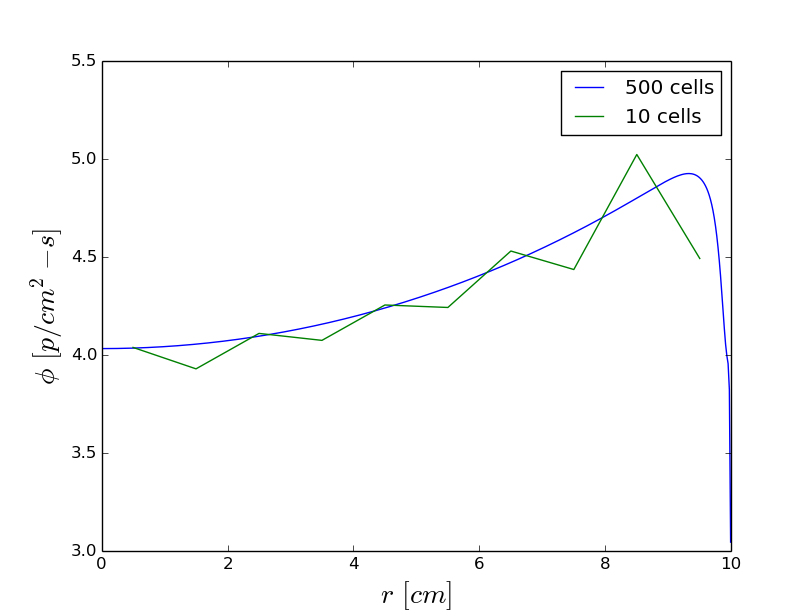
\includegraphics[width=0.6\textwidth]{final_1e.png}
    \caption{Scalar flux as a function of $r$ for part e}
    \label{fig:final_1e}
\end{figure}

As shown in Fig.(5), making the spatial discretization too coarse results in spatial oscillations. The reason for these spatial oscillations occur can be derived from equation for the starting flux
\begin{equation*}
\psi_{i-1/2,1/2}= \frac{\Big(1 - \frac{\sigma_t \Delta r}{2}\Big) \psi_{i+1/2,1/2} + Q_{i,1/2} \Delta r}{1 + \frac{\sigma_t \Delta r}{2}} \: .
\end{equation*}
By plugging in our values for $\sigma_t$ and $\Delta r$ (which are $5$ and $1$ respectively) we get
\begin{equation*}
\psi_{i-1/2,1/2}= -\frac{3}{7} \psi_{i+1/2,1/2} + \frac{2}{9} Q_{i,1/2} \: .
\end{equation*}
Thus, if $\psi_{i+1/2,1/2} > \frac{27}{14} Q_{i,1/2}$ we will get spatial oscillations for $\psi$. For this problem, these spatial oscillations will be strongest for $\mu=-1$ and $\mu_1$ because of the delta function incident flux. The simple way to get rid of these oscillations is to satisfy the following condition:
\begin{equation*}
\Big(1 - \frac{\sigma_t \Delta r}{2}\Big) > 0 
\end{equation*} 
or a slightly different version of this condition for a spherical geometry. 

\section{}

\subsection{}
The response for the forward method is
\begin{equation*}
R = \oint dA \int_{\mu>0} d\mu \, \psi(1,\mu)\mu
\end{equation*}
or using the $S_N$ code, it can be evaluated by
\begin{equation*}
R= A \sum_{m=M/2}^M \psi(1,\mu_m) \mu_m w_m \: .
\end{equation*}
Using the forward method, the $S_N$ code gives $R=4.93447$.

\subsection{}
The adjoint is defined as
\begin{equation*}
\langle q^\dagger , \psi \rangle =  \langle q , \psi^\dagger \rangle - \int_0^\infty dE \oint dA \int d\Omega \, \psi \psi^\dagger \hat{\Omega} \cdot \hat{n} \: .
\end{equation*}
For this problem the adjoint simplifies to just
\begin{equation*}
\langle q^\dagger , \psi \rangle =  \langle q , \psi^\dagger \rangle- \oint dA \int d\mu \, \psi \psi^\dagger \mu \: .
\end{equation*}
By splitting up the boundary integral into negative and positive $\mu$ values we get 
\begin{equation*}
\langle q^\dagger , \psi \rangle =  \langle q , \psi^\dagger \rangle - \oint dA \int_{\mu<0}  d\mu \, \psi \psi^\dagger \mu - \oint dA \int_{\mu>0}  d\mu \, \psi \psi^\dagger \mu \: .
\end{equation*}

Since the response for this problem is not volumetric, $q^\dagger = 0$, and since there is no source, $q=0$. In addition, since we do not automatically know what the forward flux is for $\mu > 0$, we can set $\psi^\dagger(\mu > 0) = 0$ for simplification. This leaves us with 
\begin{equation*}
R = - \oint dA \int_{\mu<0}  d\mu \, \psi \psi^\dagger \mu 
\end{equation*}
which we solve by doing an adjoint calculation. 

In the $S_N$ code, an adjoint calculation is performed by setting the extraneous source equal to $q^\dagger(-\mu)$. The solution we get from this $S_N$ calculation is $\hat{\psi}$. We can then calculate the adjoint flux by setting $\psi^\dagger(\mu) = \hat{\psi}(-\mu)$.

Thus, our response can be determine via the following inner product
\begin{equation*}
R= - A \sum_{m=1}^{M/2} \psi(1,\mu_m) \hat{\psi}(1,-\mu_m) \mu_m w_m \: .
\end{equation*}
Using adjoints, the $S_N$ code gives $R=4.93447$. The same answer as with the forward method! The reason both calculations provide the same answer is that $\psi(1,\mu_m)$ is proportional to $\hat{\psi}(1,-\mu_m)$ (the source term is zero for both, and both have an isotropic boundary condition). Also, by taking the inner product between $\psi(1,\mu_m)$ and $\hat{\psi}(1,-\mu_m)$ the solutions are renormalized to give the same result as the forward solution. 

\subsection{}

In $1^\text{st}$-order perturbation theory we start with the forward transport equation,
\begin{equation*}
\hat{L} \psi  = q
\end{equation*}
and assume each term gets perturbed some small amount  
\begin{equation*}
(\hat{L} + \delta \hat{L})(\psi + \delta \psi) = q + \delta q 
\end{equation*}
\begin{equation*}
\hat{L}\psi + \psi \delta \hat{L} + \hat{L} \delta \psi + \delta \hat{L} \delta \psi = q + \delta q  \: .
\end{equation*}
Now we eliminate $2^\text{nd}$-order terms for simplication 
\begin{equation*}
\hat{L}\psi + \psi \delta \hat{L} + \hat{L} \delta \psi = q + \delta q 
\end{equation*}
and take an inner product to get
\begin{equation}
\langle \psi^\dagger, \hat{L}\psi \rangle + \langle \psi^\dagger, \psi \delta \hat{L} \rangle + \langle \psi^\dagger,\hat{L} \delta \psi \rangle= \langle \psi^\dagger, q \rangle  + \langle \psi^\dagger,\delta q \rangle\: .
\end{equation}
Similary we can start with adjoint equation,
\begin{equation*}
\hat{L}^\dagger \psi^\dagger  = q^\dagger
\end{equation*}
and take an inner product with $\psi + \delta \psi$ to get
\begin{equation}
\langle \hat{L}^\dagger \psi^\dagger, \psi \rangle  + \langle \hat{L}^\dagger \psi^\dagger, \delta \psi \rangle = \langle \hat{L}^\dagger \psi^\dagger, q^\dagger \rangle 
\end{equation}
Next by subtracting Eq.(1) from Eq.(2) we get 
\begin{equation*}
\langle q^\dagger, \delta \psi \rangle = \langle \delta q, \psi^\dagger \rangle -  \langle \delta \hat{L} \psi, \psi^\dagger \rangle -  \int_0^\infty dE \oint dA \int d\Omega \, \delta \psi \psi^\dagger \hat{\Omega} \cdot \hat{n} 
\end{equation*}
\begin{equation}
\delta R = \langle \delta q, \psi^\dagger \rangle -  \langle \delta \hat{L} \psi, \psi^\dagger \rangle -  \int_0^\infty dE \oint dA \int d\Omega \, \delta \psi \psi^\dagger \hat{\Omega} \cdot \hat{n} 
\end{equation}
For this problem since there is only a change in $\delta \hat{L}$, Eq.(3) simplifies to 
\begin{equation*}
\delta R = - \langle \delta \hat{L} \psi, \psi^\dagger \rangle \: .
\end{equation*}
Which can be approximated with $S_N$ as 
\begin{equation*}
\delta R= - \delta \sigma_a \sum_{m=1}^{M} \sum_{i=1}^{I} \psi(1,\mu_m) \hat{\psi}(1,-\mu_m) \frac{4\pi}{3} (r_{i+1/2}^3 - r_{i-1/2}^3) w_m \: .
\end{equation*}
Thus, 
\begin{equation*}
\frac{\partial R}{\partial \sigma_a} = -\sum_{m=1}^{M} \sum_{i=1}^{I} \psi(1,\mu_m) \hat{\psi}(1,-\mu_m) \frac{4\pi}{3} (r_{i+1/2}^3 - r_{i-1/2}^3) w_m \: .
\end{equation*}
Using this forward adjoint inner product, the $S_N$ code gives $\frac{\partial R}{\partial \sigma_a}=−3.32628$. 


\subsection{}
The $1^\text{st}$-order estimate of $\delta R$ can be computed as
\begin{equation*}
\delta R =  \frac{\partial R}{\partial \sigma_a} \delta \sigma_a \: .
\end{equation*}
Thus, the $1^\text{st}$-order perturbation theory estimate is $\delta R = -0.16631$. By using two seperate $S_N$ calculations and finding the difference in the response we get that $\delta R = -0.16158$. The difference between the perturbation theory estimate and true $\delta R$ is only $2.85\%$. The reason this perturbation theory estimate isn't exact is because it is only a $1^\text{st}$-order perturbation theory estimate. In other words, we're attempting to approximate a curve using a line. Higher-order perturbation theory would have to be used in order to obtain a more accurate result for $\delta R$.



\end{document}

